\chapter{Grundlagen}
In diesem Kapitel werden die Grundlagen von Robotern behandelt. Es wird der zu Grunde liegende Aufbau des Roboters, im Bezug auf dessen Fortbewegung, vorgestellt. Ebenso werden heutige Fahrassistenzsysteme wie beispielsweise ABS vorgestellt. Zu diesem Kapitel gehört auch eine Übersicht über die Verwendung aktueller Assistenzsysteme.
\section{Bedeutung des Roboter}

\section{Antriebsart des Versuchsroboters} \label{lab:Antriebsart}
Der Versuchsroboter wird mit zwei unabhängigen Motoren ausgestattet. Diese Motoren treiben jeweils eins der beiden Haupträder an. Die Haupträder sind in der Abbildung \vref{fig:differntial} rot dargestellt. .Zusätzlich erhält der Roboter ein Stützrad, welches durch eine freilaufende Kugel realisiert wurde. Es stützt den Roboter soweit ab, dass dieser nicht nach hinten kippen kann und somit Bauteile auf dem Untergrund schleifen.
\begin{figure}[htb]
\centering
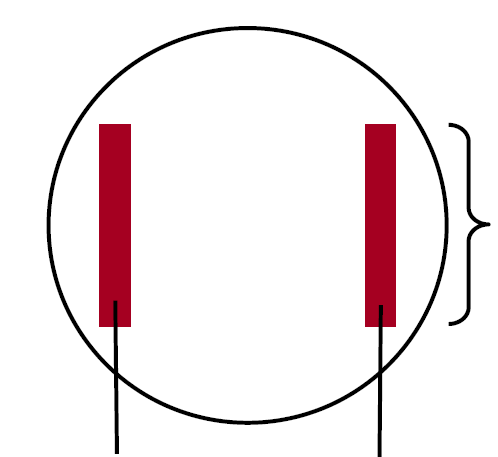
\includegraphics[width= 6cm]{Differentialantrieb}
\caption{Abstrakte Darstellung der Antriebsräder des Versuchsroboters}
\label{fig:differntial}
\end{figure}

Der Antrieb in diesem Aufbau ist ein Differential Antrieb wie in Abbildung \vref{fig:differntial} dargestellt. Mit diesem Antrieb sind sowohl Geradeausfahrten als auch Kurvenfahrten sowie das Drehen auf der Stelle möglich. Sein Hauptvorteil besteht in der einfachen Mechanik die Verbaut wird. Aufgrund seiner zwei unabhängig von einander steuerbaren Räder ist sein Einsatz für dieses Projekt optimal geeignet und sein eigentlicher Nachteil fällt somit nicht weiter auf.
 
Sein Nachteil ist, dass die Räder in Echtzeit geregelt werden müssen.  

\textbf{Quelle : Strand, Marcus Vorlesungsfolien } 

\section{Assistenzsysteme heutiger Fahrzeuge}
In der heutigen Zeit unterstützen die Fahrer einige Helfer, auch Assistenzsysteme genannt. Diese Systeme sollen dazu beitragen, den Straßenverkehr sicherer zumachen. Sie entlasten und unterstützen den Fahrer in jeglicher Fahrsituation. So helfen sie beim einparken des Fahrzeugs oder verhindern in Gefahrensituationen den Verlust über die Kontrolle.

Mit dem fortschreiten der Automobilenfortbewegung wurden immer mehr Assistenzsystem erfunden und bestehende immer weiter entwickelt. 
\subsection{ABS - Antiblockiersystem}
Ein Assistenzsystem welches sich in der Automobilbranche flächendeckend durchgesetzt hat, ist das Antiblockiersystem. Es hilft dem Fahrer, das Fahrzeug sicher zum stehen zubringen. Wie der Name schon sagt, versucht es durch gezieltes vermindern des Bremsdrucks ein blockieren des Fahrzeugs zu verhindern. Aufgrund diesen Eingriffs wird der Bremsweg verringert und der Verschleiß an den Laufflächen wird vermindert. Durch dieses System wird die Lenkbarkeit und Spurtreue erhöht.

Dieses System ist inzwischen bei jedem großen Automobilhersteller in den Ausstattungslisten der Fahrzeuge. Meist ist es serienmäßig in die Fahrzeuge integriert oder kann für einen geringen Aufpreis nachgeordert werden. 

Antiblockierysteme werden nicht nur bei Autos eingesetzt. Es wird ebenfalls in Flugzeugen Zügen und Motorrädern eingesetzt. 
Den ersten Einsatz eines solchen Systems fand 1920 in einem Flugzeug statt.

\subsection{PDC - Park Distanz Kontrolle}
Dieses System unterstützt den Fahrer mit Hilfe akustischen und visuellen Warnhinweisen beim einparken seines Fahrzeugs. 
\paragraph{Funktion}Mit Hilfe von Ultraschallsensoren, welche meist in den Heck-/Frontschürzen untergebracht sind, wird der Abstand zu Gegenständen in einer gewissen Distanz, meist ab 1-2 Meter, gewarnt. 

Diese Warnungen erfolgten bei den ersten Systemen meist akustisch über verschiedene Warntöne. Danach wurden zusätzlich kleine LED-Lampen in verschiedenen Farben eingeführt. Diese leuchten je nach Distanz zum Gegenstand oder Fahrzeug in Grün- Orange/Gelb- Rot. Die nächste Stufe ist eine optische Darstellung des Fahrzeugs auf dem Bildschirm des Infotainmentsystems. Im Bildschirm wird dann der Abstand visuell dargestellt. Zusätzlich dazu, erhält der Fahrer akustische Hinweise. Die neusten Systeme verfügen inzwischen noch über eine Kamera. Mit Hilfe der Kamera erhält der Fahrer beim einparken ein Livebild auf den Bildschirm seines Infotainmentsystems. Zusätzlich dazu wird der Abstand und der bestmögliche Fahrweg visuell im Livebild dargestellt.

Dieses System und seine Weiterentwicklungen ist die Grundlage für automatische Einparksysteme. 
\subsection{ESC-Electronic Stability Control} 
\paragraph{Geschichtliches} ESC-Electronic Stability Control ist noch ein Recht junges Assistenzsystem. Im Vergleich zum Antiblockiersystem, welches schon in 20er Jahren des 20.Jahrhunderts entwickelt und bis heute immer weiter entwickelt wurde, führte Mercedes-Benz, mit Hilfe der Bosch AG, dieses Assistenzsystem erst 1995 in der damals neu aufgelegten S-Klasse in die Serienproduktion ein. 

Der Name Elektronisches Stabilitätsprogramm (ESP) ist Eigentum der Firma Bosch. Bei anderen Herstellern gibt es ähnliche Systeme mit anderen Bezeichnungen. Bei BMW wird das System DSC-Dynamic Stability Control genannt. Bei den Herstellern von Jaguar und Mazda ist das entsprechende System ebenfalls das DSC.

Da diese unterschiedlichen Bezeichnungen zu Verwirrung führen kann wird in Fachkreisen und im Anbieter neutralen Markt meist der Begriff ESC-Electronic Stability Control oder Fahrdynamikregelung verwendet. 
\paragraph{Funktion}Dieses Assistenzsystem hilft dem Fahrer im Grenzbereich die Kontrolle seines Fahrzeuges zu behalten. 

\paragraph{Beschlüsse und Gesetze} Seit dem Beschluss des EU-Parlaments am 10.März 2009 müssen seit November 2011 alle in der EU zugelassenen Neuwagen und LKW ein entsprechendes System verwenden. Es gab eine Übergangsfrist bis Oktober 2014 für bereits zugelassene Fahrzeugtypen. Jedoch wurden Mitte 2014 immer noch einige Kleinwagen ohne ESC angeboten. 


\subsection{Automatisches einparken}

\subsection{Anwendung aktueller Assistenzsysteme}
In den Fahrzeugen, die heute die Fabrikhallen verlassen finden sich inzwischen immer mehr Assistenzsysteme. Diese reichen vom ESP bis hin zum Spurhalteassistent oder dem Automatischen Einparksystemen. Jedoch ruhen sich die Hersteller auf diesen Systemen nicht aus und entwickeln immer umfangreichere Systeme für folgende Fahrzeuggenerationen. 
\paragraph{Probleme aktueller Systeme} Bei allen Erleichterungen und aller Unterstützung für den Fahrer sollte nicht vergessen werden, dass der Fahrer immer noch selbst am Steuer sitzt und für sein Fahrzeug verantwortlich ist. Bei Testfahrten eines Erlkönigs der Marke BMW kam es am 28. März diesen Jahres zu einem Unfall. Während der Testfahrt, auf der der Fahrer laut dem Hersteller \textbf{„kamerabasierte“ Fahrerassistenzsysteme bei Dunkelheit testen} sollte kam es in Stuttgart zu einem Unfall. In diesen Unfall war ein, mit Sondersignal fahrendes, Polizeiauto verwickelt, welches im Kreuzungsbereich durch den Zusammenstoß umkippte.
Dieser Unfall zeigt, dass die heutigen Assistenzsysteme schon sehr weit entwickelt sind. Jedoch bedarf es immer noch einem Fahrer, der in Ausnahmesituationen eingreifen kann und einen solchen Unfall verhindert. Weshalb der Fahrer in dieser Situation nicht eingegriffen hat, oder ob es ein Problem mit der Steuerung gab ist nicht bekannt.

Wie dieser Unfall zeigt sind die Assistenzsysteme noch nicht soweit, dass sie alleine, ohne Fahrer, im Straßenverkehr bestehen können. 

\paragraph{Zukunftsweißende Projekte} Jedoch sind die Hersteller inzwischen soweit, dass sie Fahrzeuge im Testbetrieb haben, die ohne Fahrer ihre Runden auf den Rennstrecken dieser Welt drehen können. So stellte AUDI, im Rahmen des letzten DTM-Rennens der Saison 2014, ein Auto (Abbildung\vref{fig:audicar}) vor, welches ohne Fahrer eine Runde im Renntempo über den Hockenheimring fuhr. Die Daten für den Fahrtweg ermittelt es mithilfe von Kameras, die in und um das Fahrzeug verteilt sind. Unterstützt wird es durch weitere Sensoren wie GPS, Raddrehzahlsensor, Gierratensensor und andern Sensoren. Aus diesen Daten errechnet der Computer die Optimale Geschwindigkeit, Bremspunkte und Position auf der Strecke. Bei den Zuschauern kam diese Vorführung gut an. Das Fahrzeug wurde in der Zwischenzeit in mehreren Fernsehsendungen, unter anderem bei GRIP auf RTL II, vorgestellt. 
\begin{figure}[htb]
\centering
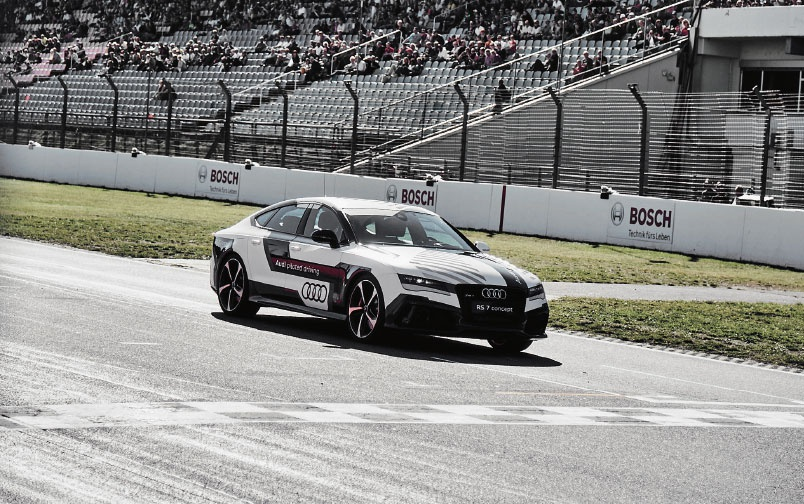
\includegraphics[width= 15cm]{audicar}
\caption{Selbst fahrender AUDI RS7 auf dem Hockenheim 2014 }
\label{fig:audicar}
\end{figure}
\textbf{Quelle Bild: \url{ http://audi-encounter.com/de/img/article-image-main/2015_1_Bobby_Car_Gallery_09.jpg_2130.jpg}}


Ein ähnliches Auto hat auch BMW im Fuhrpark. Dieses Fahrzeug wurde in der Sendung TopGear mit Jeremy Clarkson vorgestellt und getestet, jedoch ist dieses Fahrzeug weit weniger bekannt als das von AUDI.

Trotz dem Erfolg dieser Autos auf den Rennstrecken, darf nicht vergessen werden, dass diese Systeme in dieser Konstellation nicht auf öffentlichen Straßen verwendet werden dürfen. Jedoch arbeiten die Hersteller intensiv daran, den Fahrer immer mehr zu entlasten und ihm bei kritischen Situationen zu unterstützen. So werden auch Systeme für den Stop-and-Go Verkehr getestet. Ein solches System soll dem Fahrer entlasten. Es übernimmt innerhalb dieser Fahrsituation gewisse Aufgaben des Fahrers.

\paragraph{Fazit} Heutige Fahrassistenzsysteme unterstützen den Fahrer in Gefahrensituationen wie beispielsweise mit ESP für schleudernde Fahrzeuge oder einem Notbremssystem für Fußgänger. Ebenso helfen sie dem Fahrer durch vollautomatisches oder teil-automatisiertes einparken. 

Trotz der Fülle verschiedener Assistenzsysteme ist  immer noch ein Fahrer nötig, der das Fahrzeug steuert. 




\section{Automatisch geführte Fahrzeuge}
